\documentclass[addpoints,12pt]{exam}
\usepackage{setspace}
\usepackage[a4paper,bindingoffset=0cm, left=3cm, right=2.5cm, top=4cm, bottom=2cm, footskip=0.5cm]{geometry}
\usepackage{amsmath,amsfonts,amssymb,mathtools}
\usepackage{listings}
\usepackage{tikz}
\usepackage{fancybox}
\usepackage{multicol}
\definecolor{blue}{rgb}{0.1,0.5,0.4}
\usepackage{wasysym}
\usepackage{pifont}
\usepackage{polyglossia}
\usepackage{ulem}
%===============================================================
% Change the font to what you prefer ...

\setdefaultlanguage[calendar=gregorian,locale=algeria]{arabic}
\setotherlanguage[variant=british]{english}
\newfontfamily\arabicfont[Script=Arabic,Scale=1.1]{Amariya}
\newfontfamily\arabicfontsf[Script=Arabic,Scale=1.1]{Amariya}
\newfontfamily\arabicfonttt[Script=Arabic,Scale=1.1]{Amariya}


% w/o following space!
\newcommand{\quem}{\tikz[baseline=(wi.base)]{\node[fill=black,rotate=45,inner sep=.1ex, text height=1.3ex, text width=1.3ex] {};%
\node[ font=\color{white}] (wi) {?};}}

\makeatletter
\renewcommand{\eqref}[1]{(\textup{{\ref{#1}}})}

%------------------------------
\pointsinmargin
%\pointsinrightmargin
\marginpointname{درجات}
\pointformat{\fbox{\bfseries\boldmath\themarginpoints}}
\setlength{\marginpointssep}{1.8cm}
\setlength{\rightpointsmargin}{1.5cm}
\renewcommand{\thepartno}{\arabic{partno}}
\renewcommand{\thesubpart}{\Alph{subpart}}
\renewcommand\subpartlabel{\thesubpart)}
\renewcommand\partlabel{\thepartno)}
\renewcommand{\partshook}{\setlength{\topsep}{-0.2in}}
\setlength{\headsep}{1pt}
\baselineskip = 0.9cm
\pointpoints{نقطة}{نقاط}
%\emph{}\qformat{\textbf{\uline{\sffamily{  التـمرين   \thequestion :}}}\quad (\thepoints)\hfill}
%---------------------------------------

\pagestyle{headandfoot}
\firstpageheadrule
\firstpageheader{صفحة $\thepage$}{ }{الإسم:}
\firstpagefooter{}{$\blacklozenge \blacklozenge$ تأكد من تظليل الإجابة على صفحة
الغلاف $\blacklozenge \blacklozenge$}
{}
\firstpagefootrule
\runningheader{صفحة $\thepage$}{ }{الإسم:}
\runningfooter{}
{$\blacklozenge \blacklozenge$ تأكد من تظليل الإجابة على صفحة
الغلاف $\blacklozenge \blacklozenge$}
{}
\runningheadrule
\runningfootrule
\setlength{\headsep}{-0.01in}

%%%%% Cover page
%
\coverfirstpageheader
{مادة معادلات تفاضلية عادية \\ الإختبار الدوري الأول \\ الزمن: ساعة}
{
{
\includegraphics[width=2.7cm]{logo1.jpg}}
}
{جامعة الطائف \\ قسم الرياضيات \\ و الإحصاء}
\runningheadrule
\runningfootrule
\onehalfspacing

\makeatother


%=============user defined command ==============
\begin{document}


\pointformat{(\thepoints)}
\pointsinrightmargin
\boxedpoints   % or \bracketedpoints

\begin{coverpages}
\hrule
\hrule
\noindent
\\ \\
\centering
\shadowbox{
\begin{minipage}{6.in}
\begin{tabular}{@{}p{.55\textwidth}@{\hspace{2cm}}p{.30\textwidth}@{}}
الإسم:\enspace\hrulefill & الرقم الجامعي:\enspace\hrulefill \\
الرقم التسلسلي: \enspace\hrulefill &
\end{tabular}
\noindent
\vspace{0.5cm}
\end{minipage}
}
\vspace{1.2cm}

\shadowbox{
\begin{minipage}{6.in}
\centering
\underline{\large{\textbf{تعليمات}}}
\begin{itemize}
  \item تأكد من كتابة إسمك أعلى كل ورقة في المكان المخصص لذلك.
  \item تأكد من إقفال الهاتف الجوال، و عدم حمل أي شيء يتعلق بالمادة.
  \item ضرورة الإلتزام بالهدوء داخل القاعة، و طلب الإذن من المراقب في حال وجود أية استفسار لديك.
  \item تأكد من تضليل الإجابة الصحيحة في المكان المخصص لذلك على صفحة الغلاف.
  \item تأكد أن عدد الصفحات هو \textbf{\totalnumpages \:} صفحات.
%  \item يمكن إستخدام الصفحات البيضاء كهوامش للحل.
\end{itemize}
\end{minipage}
}
\begin{figure}[hhh!]
\centering
    {\selectlanguage{english}\resizebox{.55\textwidth}{!}{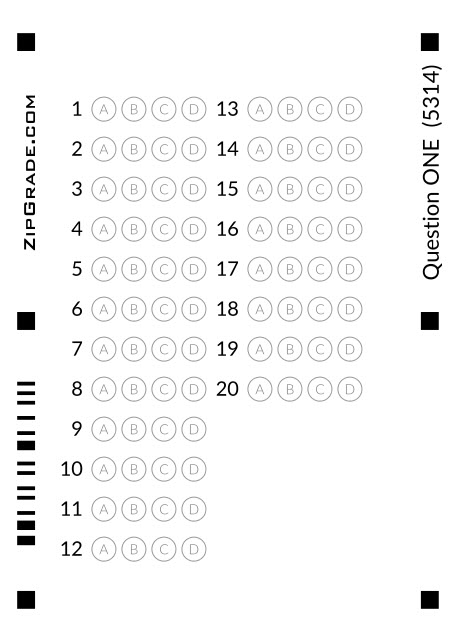
\includegraphics{NA_Multiple.jpg}}}
    \end{figure}

\end{coverpages}

\fontsize{14pt}{14pt}\selectfont

أجب عما يلي

\begin{questions}

\question \uplevel{ إعتبر المعادلة التفاضلية
\begin{equation}\label{ode.1}
  \displaystyle y''^2 + 5y+ 6y = 0
\end{equation}
} رتبة المعادلة التفاضلية  \eqref{ode.1} هي

\begin{oneparchoices}
\selectlanguage{english}
\choice $2$
\choice $1$
\choice $0$
\CorrectChoice $3$
\end{oneparchoices}
\question[4] أجب عما يلي
\begin{parts}
\item أوجد مشتقة الدالة $f(x)$.
\fillwithdottedlines{1in}
\item أوجد مشتقة الدالة $g(x)$.
\fillwithdottedlines{1in}
\end{parts}

\question[6]
إحسب $\displaystyle \int_0^5 e^{x}\: dx$.
\fillwithdottedlines{1.6in}

\question[5]
إرسم الدالة $g(x)= \tan(x)$\\
\fillwithdottedlines{1.8in}

\question
إعتبر النظام الخطي التالي
\begin{align*}
\nonumber   x_1 - x_2 + x_3 &= 1 \\
\nonumber  x_1 + x_2 + x_3&= 2 \\
\nonumber  x_1 + 3x_2 + x_3 &= 21
\end{align*}

أوجد حل النظام بإستخدام
\begin{parts}
\part[5] طريقة كرامر.
\fillwithdottedlines{3.in}
\part[5] طريقة جاوس - سيدال التكرارية
\fillwithdottedlines{3.in}
\end{parts}


\end{questions}

\begin{center}
\fbox{\fbox{\parbox{5.5in}{\centering
مع تمنياتي لكم بخالص التوفيق و السداد!}}}
\end{center}
\end{document}

%%% Local Variables:
%%% mode: latex
%%% TeX-master: t
%%% End:
